\documentclass{article}
\usepackage{amsmath}
\usepackage{tikz}
\usetikzlibrary{arrows.meta, calc}

\begin{document}
	
	\section{Intersection of a ray with a triangle}
	
	This implementation uses the Möller–Trumbore intersection algorithm.
	
	Given a ray defined by its origin \(\mathbf{o}\) and direction \(\mathbf{d}\), and a triangle defined by its vertices p1, p2, and p3:
	
	\subsection{Compute the edge vectors}
	
	
	
	\[
	\mathbf{e1} = p2 - p1
	\]
	
	
	
	
	\[
	\mathbf{e2} = p3 - p1
	\]
	
	
	
	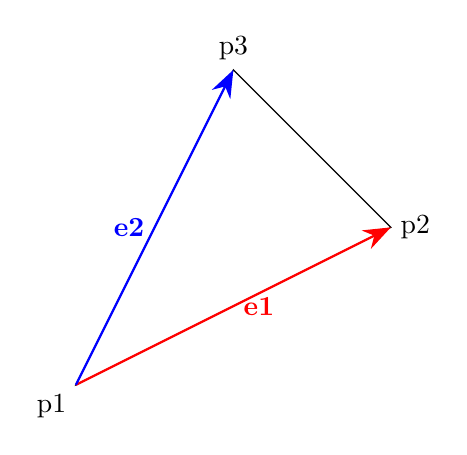
\begin{tikzpicture}[scale=2]
		\coordinate (p1) at (0,0);
		\coordinate (p2) at (2,1);
		\coordinate (p3) at (1,2);
		\draw (p1) -- (p2) -- (p3) -- cycle;
		\draw [-{Stealth[scale=1.5]},thick,red] (p1) -- (p2) node[midway,right] {$\mathbf{e1}$};
		\draw [-{Stealth[scale=1.5]},thick,blue] (p1) -- (p3) node[midway,left] {$\mathbf{e2}$};
		\node[below left] at (p1) {p1};
		\node[right] at (p2) {p2};
		\node[above] at (p3) {p3};
	\end{tikzpicture}
	
	\subsection{Compute the determinant w}
	
	
	
	\[
	\mathbf{l} = \mathbf{d} \times \mathbf{e2}
	\]
	
	
	
	
	\[
	\mathbf{w} = \mathbf{e1} \cdot \mathbf{l}
	\]
	
	
	
	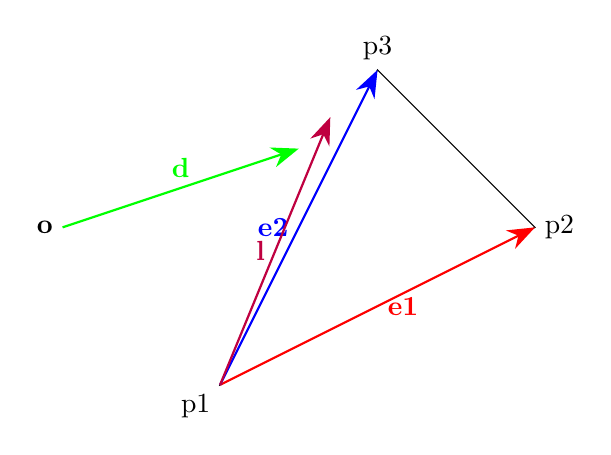
\begin{tikzpicture}[scale=2]
		\coordinate (p1) at (0,0);
		\coordinate (p2) at (2,1);
		\coordinate (p3) at (1,2);
		\coordinate (o) at (-1,1);
		\draw (p1) -- (p2) -- (p3) -- cycle;
		\draw [-{Stealth[scale=1.5]},thick,green] (o) -- ($(o)+(1.5,0.5)$) node[midway,above] {$\mathbf{d}$};
		\draw [-{Stealth[scale=1.5]},thick,red] (p1) -- (p2) node[midway,right] {$\mathbf{e1}$};
		\draw [-{Stealth[scale=1.5]},thick,blue] (p1) -- (p3) node[midway,left] {$\mathbf{e2}$};
		\draw [-{Stealth[scale=1.5]},thick,purple] (p1) -- ($(p1)+(0.7,1.7)$) node[midway,left] {$\mathbf{l}$};
		\node[below left] at (p1) {p1};
		\node[right] at (p2) {p2};
		\node[above] at (p3) {p3};
		\node[left] at (o) {$\mathbf{o}$};
	\end{tikzpicture}
	
	If \(\mathbf{w}\) is near zero, the ray lies in the plane of the triangle.
	
	\subsection{Compute the inverse determinant i}
	
	
	
	\[
	i = \frac{1}{\mathbf{w}}
	\]
	
	
	
	\subsection{Compute the distance vector}
	
	
	
	\[
	\mathbf{t} = \mathbf{o} - p1
	\]
	
	
	
	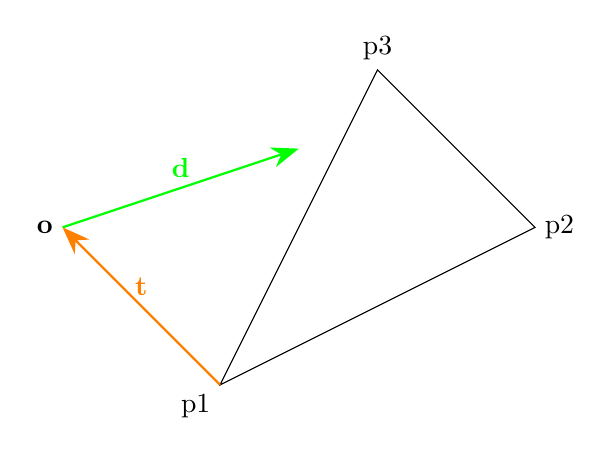
\begin{tikzpicture}[scale=2]
		\coordinate (p1) at (0,0);
		\coordinate (p2) at (2,1);
		\coordinate (p3) at (1,2);
		\coordinate (o) at (-1,1);
		\draw (p1) -- (p2) -- (p3) -- cycle;
		\draw [-{Stealth[scale=1.5]},thick,green] (o) -- ($(o)+(1.5,0.5)$) node[midway,above] {$\mathbf{d}$};
		\draw [-{Stealth[scale=1.5]},thick,orange] (p1) -- (o) node[midway,above] {$\mathbf{t}$};
		\node[below left] at (p1) {p1};
		\node[right] at (p2) {p2};
		\node[above] at (p3) {p3};
		\node[left] at (o) {$\mathbf{o}$};
	\end{tikzpicture}
	
	\subsection{Compute the \(u\) parameter}
	
	
	
	\[
	u = (\mathbf{t} \cdot \mathbf{l}) \times i
	\]
	
	
	
	\subsection{Compute the \(v\) parameter}
	
	
	
	\[
	\mathbf{q} = \mathbf{t} \times \mathbf{e1}
	\]
	
	
	
	
	\[
	v = (\mathbf{d} \cdot \mathbf{q}) \times i
	\]
	
	
	
	\subsection{Compute the intersection distance}
	
	
	
	\[
	t = (\mathbf{e2} \cdot \mathbf{q}) \times i
	\]
	
	
	
	This algorithm efficiently determines if a ray intersects with a triangle by using barycentric coordinates and vector mathematics. It ensures that the intersection point lies within the triangle and not just on the plane of the triangle.
	
\end{document}
